\section{Graphical Design}

Based on our analysis, it turns out that there does not seem to be a relation between the complexity of the graphics, and the impact this has on how 
much fun, the game is or how educating the game is. For this reason 2D graphics has been deemed sufficient for this game. The following section will go 
through the design choices that has been made in terms of the graphical interface of the game, along with justification for why a given choice was made.

\subsection{World Map}

The world map is a hexagon consisting of smaller 'cells' which are also hexagonal. This means that by design the entire field is hexagonal. A cell takes 
up a single small-hexagon on the field, and as does the various food types.


\begin{figure}[h]
	\centering
		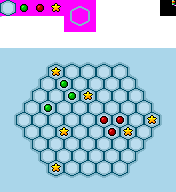
\includegraphics{img/cells_mockup.png}
	\caption{Playing field with cells and food}
	\label{fig:cells_mockup}
\end{figure}